\section{External Interface Requirements}
\subsection{User Interfaces}
The S\&C user interfaces will consist of a website and a mobile application. The website will primarily be used by companies and students, e.g., to upload their CVs and edit their profiles. The mobile application, however, will be particularly useful for students who want to quickly check their inbox or monitor section. At least one interface will be accessible to anyone with an Internet connection and a compatible device.
\subsection{Hardware Interfaces}
For hardware interfaces, users can choose between a computer (with a browser) or a mobile device, such as a smartphone or tablet, with the mobile application installed. Every device will have to be connected to the Internet.
\subsection{Software Interfaces}
The system requires the Revenue Agency's API to verify the validity of a company's data. It also uses universities' SSO to manage student login. Additionally, it includes an admin dashboard for reviewing company registrations, responding via email, and monitoring user feedback.
\subsection{Communication Interface}
The platform ensures secure and efficient communication through a combination of protocols. HTTPS encrypts all data transmitted between clients and servers, ensuring confidentiality and integrity. RESTful APIs are used to integrate with external systems such as the Revenue Agency and university SSO. Secure messaging is achieved through WebSocket connections encrypted with TLS, enabling real-time communication. Finally, Firebase Cloud Messaging (FCM) ensures reliable push notifications to mobile devices.
\section{Functional Requirements}

\textbf{Sign up and Log in}
\begin{itemize}
    \item[\text{[R1]}] S\&C allows Students to sign up to the platform through their university credentials using SSO access.
    \item[\text{[R2]}] S\&C allows Student to login via their university credentials.
    \item[\text{[R3]}] S\&C allows Companies to sign up to the platform by asking the representative of the company to insert their company email, the VAT number of the company, a Certificate of registration at the Chamber of Commerce, and a letter of authorisation or official assignment signed by a CEO or a HR referent. They have to choose a password.
    \item[\text{[R4]}] S\&C allows Companies to login to the platform via password and username (created by the system).
    
\end{itemize}

\textbf{Update Student's profile}
\begin{itemize}
    \item[\text{[R5]}] S\&C allows Students to upload the PDF of their CV (both for the first time and other times if there have been some changes).
    \item[\text{[R6]}] S\&C allows Students to insert new experiences, skills, and attitudes on their profile.
    \item[\text{[R7]}] S\&C allows Students to edit or delete experiences, skills, and attitudes present on their profile.
\end{itemize}

\textbf{Create internship's advertisement}
\begin{itemize}
    \item[\text{[R8]}] S\&C allows Companies to create an advertisement regarding an internship position they are offering, explaining the project of the internship and the terms offered.

    \item[\text{[R9]}] S\&C allows Companies to modify and remove an advertisement posted on their page.
\end{itemize}

\textbf{Proactive research}
\begin{itemize}
    \item[\text{[R10]}] S\&C allows Students to use a research bar to find appropriate internship positions by inserting specific requirements about the project and/or the terms offered.
    
    \item[\text{[R11]}] S\&C allows Companies to use a research bar to find appropriate candidates for their internship positions by inserting specific experiences, skills and/or attitudes the candidates should have.
\end{itemize}

\textbf{Recommendation}
\begin{itemize}
    \item [\text{[R12]}] S\&C informs students when an internship that might interest them becomes available.

    \item [\text{[R13]}] S\&C informs companies about the availability of a student whose CV corresponds to their needs.
\end{itemize}

\textbf{Matchmaking between company and student and establishment of a contact}
\begin{itemize}
    \item [\text{[R14]}] S\&C allows Students to contact a company they are interested in.
    
    \item [\text{[R15]}] S\&C allows Companies to contact Students they are interested in.

    \item [\text{[R16]}] S\&C informs a Student when a Company shows interest in their profile by sending the Student the Company's offer. The Student can accept or decline the offer.

    \item [\text{[R17]}] S\&C informs a Company when a Student shows interest in its offer by sending to the Company the Student's CV, the Company can accept or decline the offer.

    \item [\text{[R18]}] S\&C communicates to Students or Companies if their requests are successful.
\end{itemize}

\textbf{Selection process}
\begin{itemize}
    \item [\text{[R19]}] S\&C allows Companies to setup an interview with the candidates.

    \item [\text{[R20]}] S\&C allows Companies to write a form with all the aspects that will be considered during the interviews.

    \item [\text{[R21]}] S\&C allows Companies to modify or delete the interview form created.

    \item [\text{[R22]}] S\&C allows Companies fill the form during the interview.
\end{itemize}

\textbf{Feedback}
\begin{itemize}
    \item [\text{[R23]}] S\&C allows Students to give personal feedback during the selection period about the Company's selection method or during the internship period about the internship itself.

    \item [\text{[R24]}] S\&C allows Companies to give feedback during the internship about a single Student.
\end{itemize}

\textbf{Monitoring of the matchmaking process}
\begin{itemize}
    \item [\text{[R25]}] S\&C offers Students the possibility to monitor their matchmaking process with a Company (state of the matchmaking, scheduled interview, interview results).

    \item [\text{[R26]}] S\&C offers Companies the possibility to monitor their matchmaking process with a Student.

    \item [\text{[R27]}] S\&C offers Students and Companies the possibility to monitor the state of the internship.
\end{itemize}

\subsection{Use Case Diagram}

\begin{figure}[H]
    \centering
    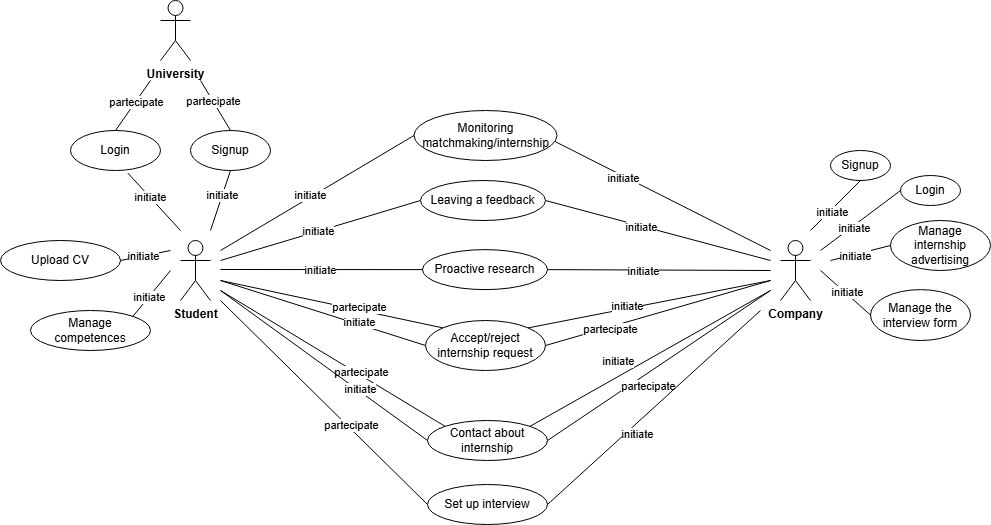
\includegraphics[width=15cm]{Images/usecasediagram2.png}
    \caption{Use Case Diagram}
\end{figure}

\subsection{Use Cases}

% Contatore
\newcounter{useCasesCounter}

\newcommand{\nextUseCases}{\stepcounter{useCasesCounter}\arabic{useCasesCounter}}

\textbf{[UC\nextUseCases] Students Signup}
\begin{table}[H] %per metterla esattamente dopo il titoletto
    \centering
    \begin{tabular}{|p{3cm}|p{10cm}|} 
    \hline
    Name & Students Sign up \\ \hline
    Actor  & Student, University website\\ \hline
    Entry Condition  & A university student wants to use the platform, they are in the login page but they are not registered \\ \hline
    Event Flow  & 
    \begin{enumerate}[noitemsep, topsep=0pt]
        \item In the login page the user finds the button “Sign up”.
        \item The students clicks on it and it opens a form.
        \item In the form the student has to insert their own university email and their university (selected via a drop down menu).
        \item They click on the button “SSO login”.
        \item They are redirected to their university login page.
        \item They accept the terms and conditions.
    \end{enumerate} \\ \hline
    Exit Condition  & The student is registered and can access the platform \\ \hline
    Exception  & (4) The email is wrong or does not correspond to the university inserted. The system inserts an error message near the input insertion bar of the email. \\ \hline
    Special Reqs  & - \\ \hline
    \end{tabular}
    \caption{[UC1] Students Signup}
\end{table}

\textbf{[UC\nextUseCases] Students Login}
\begin{table}[H] %per metterla esattamente dopo il titoletto
    \centering
    \begin{tabular}{|p{3cm}|p{10cm}|} 
    \hline
    Name & Students Login \\ \hline
    Actor  & Student, University website\\ \hline
    Entry Condition  & The student is on the login page and wants to access the platform. \\ \hline
    Event Flow  & 
    \begin{enumerate}[noitemsep, topsep=0pt]
        \item The student insert their own university email.
        \item They click on the “Login” button.
        \item They are redirected to their university login page.
    \end{enumerate} \\ \hline
    Exit Condition  & The student is logged in. \\ \hline
    Exception  & (2) The email is wrong or the student is not registered to the platform. The system inserts an error message near the input insertion bar of the email. \\ \hline
    Special Reqs  & - \\ \hline
    \end{tabular}
    \caption{[UC2] Students Login}
\end{table}

\textbf{[UC\nextUseCases] Company Sign up}
\begin{table}[H] %per metterla esattamente dopo il titoletto
    \centering
    \begin{tabular}{|p{3cm}|p{10cm}|}
    \hline
    Name & Company Sign up \\ \hline
    Actor  & Company \\ \hline
    Entry Condition  & A representative of a company wants to use the platform, they are in the login page but they are not registered. \\ \hline
    Event Flow  & 
    \begin{enumerate}[noitemsep, topsep=0pt]
        \item In the login page the user finds the button “Sign up”.
        \item The user clicks on it and they are redirected to a form.
        \item They have to insert the company’s data: name and VAT number, and upload a Certificate of registration at the Chamber of Commerce. They must also verify their authorisation to register the company by providing their official company email and uploading an authorisation letter or an official assignment signed by the CEO or an HR representative.
        \item They click on the “Submit” button.
        \item They will receive an email that confirms the registration, the mail contains a username chosen by the system and a link to setup a password.
        \item The user clicks on the link and sets up a password according to the rules stated on the page (minimum and maximum length, alphanumeric…).
    \end{enumerate} \\ \hline
    Exit Condition  & The Company is registered and now can access the platform. \\ \hline
    Exception  & 
    \begin{itemize}
        \item [\text{(4)}] The VAT number is not valid (check done with the Revenue Agency’s API). The system inserts an error message near the input insertion bar of the VAT number.
        \item [\text{(4)}] The email is wrong or does not correspond to the company inserted. The system inserts an error message near the input insertion bar of the email.
        \item [\text{(5)}] The documentation uploaded is not valid (checks done by the S\&C’s employees). The employees send an email to the representative explaining the documentation is not valid and send an email to the official company warning them about a possible forgery of their documentation.
        \item [\text{(6)}] The password is not valid because it does not check all requirements. The system inserts an error message near the input insertion bar of the password.
    \end{itemize}
    \\ \hline
    Special Reqs  & The manual checking of the documentation has to be done in less then 3 working days. \\ \hline
    \end{tabular}
    \caption{[UC3] Company Sign up}
\end{table}

\textbf{[UC\nextUseCases] Company Login}
\begin{table}[H] %per metterla esattamente dopo il titoletto
    \centering
    \begin{tabular}{|p{3cm}|p{10cm}|}
    \hline
    Name & Company Login \\ \hline
    Actor  & Company\\ \hline
    Entry Condition  & A representative of a company wants to login to the platform, they are in the login page. \\ \hline
    Event Flow  & 
    \begin{enumerate}[noitemsep, topsep=0pt]
        \item In the login page the user inserts the username and the password.
        \item The user clicks on “Login”.
    \end{enumerate} \\ \hline
    Exit Condition  & The user is logged in. \\ \hline
    Exception  & 
    \begin{itemize}
        \item [\text{(2)}] The credentials are empty. The system shows error messages near the fields to be filled.
        \item [\text{(2)}] The credentials are wrong. The system shows a pop-up window asking to re-insert them.
    \end{itemize}
    \\ \hline
    Special Reqs  & The manual checking of the documentation has to be done in less than 3 working days. \\ \hline
    \end{tabular}
    \caption{[UC4] Company Login}
\end{table}

\textbf{[UC\nextUseCases] Update student’s CV}
\begin{table}[H] %per metterla esattamente dopo il titoletto
    \centering
    \begin{tabular}{|p{3cm}|p{10cm}|}
    \hline
    Name & Update student’s CV \\ \hline
    Actor  & Student \\ \hline
    Entry Condition  & The student is on their page and wants to upload a new CV \\ \hline
    Event Flow  & 
    \begin{enumerate}[noitemsep, topsep=0pt]
        \item The student clicks on the “Upload new CV” button.
        \item The student inserts the pdf of their CV using the drag and drop function, by selecting the correct local directory.
    \end{enumerate}
    \\ \hline
    Exit Condition  &  The CV is correctly uploaded on the personal page of the student. \\ \hline
    Exception  & (2) The CV’s dimension is too large. The system shows a pop-up window asking to upload a lighter pdf. \\ \hline
    Special Reqs  & -- \\ \hline
    \end{tabular}
    \caption{[UC5] Update student’s CV}
\end{table}

\textbf{[UC\nextUseCases] Insert Student’s experiences, skills and/or attitudes.}
\begin{table}[H] %per metterla esattamente dopo il titoletto
    \centering
    \begin{tabular}{|p{3cm}|p{10cm}|}
    \hline
    Name & Insert Student’s experiences, skills and/or attitudes. \\ \hline
    Actor  & Student \\ \hline
    Entry Condition  & The user is in their own profile page and wants to insert personal experiences, skills and/or attitudes. \\ \hline
    Event Flow  & 
    \begin{enumerate}[noitemsep, topsep=0pt]
        \item The user clicks on the button “Insert new competence”.
        \item The user is redirected to a form.
        \item They have to select the type of competence through a drop-down menu (experience, skill, attitude), then they can click on the suggested competence or they can simply write it. Optionally, they can add a note to explain it.
        \item They can click on the “plus” icon to add another competence.
        \item When they finish, they click on the button “Done”.
    \end{enumerate}
    \\ \hline
    Exit Condition  & The new competences are uploaded to their profile. \\ \hline
    Exception  & (5) The user has inserted something inappropriate, so the system shows a pop-up. \\ \hline
    Special Reqs  & If the user changes their mind, they can click on the “cross” icon and go back to their profile. \\ \hline
    \end{tabular}
    \caption{[UC6] Insert Student’s experiences, skills and/or attitudes.}
\end{table}

\textbf{[UC\nextUseCases] Edit or delete Student’s experiences, skills and/or attitudes.}
\begin{table}[H] %per metterla esattamente dopo il titoletto
    \centering
    \begin{tabular}{|p{3cm}|p{10cm}|}
    \hline
    Name & Edit or delete Student’s experiences, skills and/or attitudes. \\ \hline
    Actor  & Student \\ \hline
    Entry Condition  & The user is in their own profile page and wants to edit personal experiences, skills and/or attitudes. \\ \hline
    Event Flow  & 
    \begin{enumerate}[noitemsep, topsep=0pt]
        \item The user clicks on the button “Edit competences”.
        \item The user is redirected to a form.
        \item They have to select the competence they want to edit through a drop-down menu. Then they can edit it or remove it.
        \item They can click on the “plus” icon to edit another competence.
        \item When they finish, they click on the button “Done”.
    \end{enumerate}
    \\ \hline
    Exit Condition  &  The competences are updated. \\ \hline
    Exception  & (5) The user has inserted something inappropriate, so the system shows a pop-up with an error message. \\ \hline
    Special Reqs  & If the user changes their mind, they can click on the “cross” icon and go back to their profile. \\ \hline
    \end{tabular}
    \caption{[UC7] Edit or delete Student’s experiences, skills and/or attitudes.}
\end{table}

\textbf{[UC\nextUseCases] Create internship advertising}
\begin{table}[H] %per metterla esattamente dopo il titoletto
    \centering
    \begin{tabular}{|p{3cm}|p{10cm}|}
    \hline
    Name & Create internship advertising \\ \hline
    Actor  & Company \\ \hline
    Entry Condition  & The user is on their profile page and wants to create an advertising. \\ \hline
    Event Flow  & 
    \begin{enumerate}[noitemsep, topsep=0pt]
        \item The user clicks on the button “Create new internship advertising”.
        \item The user is redirected to a form.
        \item They have to insert: name of the the internship position, location, profile they are looking for, project description (application domain, tasks to be performed, relevant adopted technologies, etc), terms offered (retribution, benefits, mentorship, …). 
        \item When they finish, they click on the button “Done”.
    \end{enumerate}
    \\ \hline
    Exit Condition  & The advertising is correctly posted. \\ \hline
    Exception  & (4) Some fields are missing, the system shows an error message near the input insertion bar. \\ \hline
    Special Reqs  & - \\ \hline
    \end{tabular}
    \caption{[UC8] Create internship advertising}
\end{table}

\textbf{[UC\nextUseCases.1] Edit internship advertising}
\begin{table}[H] %per metterla esattamente dopo il titoletto
    \centering
    \begin{tabular}{|p{3cm}|p{10cm}|}
    \hline
    Name & Edit internship advertising \\ \hline
    Actor  & Company \\ \hline
    Entry Condition  & The user is on the advertising page and wants to edit it. \\ \hline
    Event Flow  & 
    \begin{enumerate}[noitemsep, topsep=0pt]
        \item The user clicks on the button “Edit”.
        \item The user is redirected to a form.
        \item They edit the desired field.
        \item When they finish, they click on the button “Done”.
    \end{enumerate}
    \\ \hline
    Exit Condition  & The advertising is correctly updated. \\ \hline
    Exception  & (4) Some fields are missing, the system shows an error message near the input insertion bar. \\ \hline
    Special Reqs  & - \\ \hline
    \end{tabular}
    \caption{[UC9.1] Edit internship advertising}
\end{table}

\textbf{[UC9.2] Remove internship advertising}
\begin{table}[H] %per metterla esattamente dopo il titoletto
    \centering
    \begin{tabular}{|p{3cm}|p{10cm}|}
    \hline
    Name & Remove internship advertising \\ \hline
    Actor  & Company \\ \hline
    Entry Condition  & The user is on the advertising page and wants to remove it. \\ \hline
    Event Flow  & 
    \begin{enumerate}[noitemsep, topsep=0pt]
        \item The user clicks on the button “Delete”.
        \item The system shows a pop-up window with a confirmation message.
        \item The user clicks on the “I am sure” button.
    \end{enumerate}
    \\ \hline
    Exit Condition  & The advertising is correctly removed. \\ \hline
    Exception  & - \\ \hline
    Special Reqs  & If the user clicks on the “Back” button the advertising remains online. \\ \hline
    \end{tabular}
    \caption{[UC9.2] Remove internship advertising}
\end{table}

\textbf{[UC\nextUseCases] Proactive internship research}
\begin{table}[H] %per metterla esattamente dopo il titoletto
    \centering
    \begin{tabular}{|p{3cm}|p{10cm}|}
    \hline
    Name & Proactive internship research \\ \hline
    Actor  & Student \\ \hline
    Entry Condition  & The user clicks on the research bar to find an internship \\ \hline
    Event Flow  & 
    \begin{enumerate}[noitemsep, topsep=0pt]
        \item The user inserts the desired characteristics in the research bar (such as details of the project and or terms).
        \item The system shows the correspondent internships (if any).
        \item The user can click on the showed internship to visit the advertise page and or the company profile.
        \item The Student can contact the Company by writing a short message
    \end{enumerate}
    \\ \hline
    Exit Condition  & The user concludes its research. \\ \hline
    Exception  & - \\ \hline
    Special Reqs  & - \\ \hline
    \end{tabular}
    \caption{[UC10] Proactive internship research}
\end{table}

\textbf{[UC\nextUseCases] Proactive candidates research}
\begin{table}[H] %per metterla esattamente dopo il titoletto
    \centering
    \begin{tabular}{|p{3cm}|p{10cm}|}
    \hline
    Name & Proactive candidates research\\ \hline
    Actor  & Company  \\ \hline
    Entry Condition  & The user clicks on the research bar to find candidates \\ \hline
    Event Flow  & 
    \begin{enumerate}[noitemsep, topsep=0pt]
        \item The user inserts the desired characteristics in the research bar (such skills, experiences and/or attitudes).
        \item The system shows the correspondent Student profiles (if any).
        \item The user can click on the shown profiles and contact the Student by writing a short message
    \end{enumerate}
    \\ \hline
    Exit Condition  & The user concludes its research. \\ \hline
    Exception  & - \\ \hline
    Special Reqs  & - \\ \hline
    \end{tabular}
    \caption{[UC11] Proactive candidates research}
\end{table}

\textbf{[UC\nextUseCases-\nextUseCases-\nextUseCases-\nextUseCases] Consult Recommendations}
\begin{table}[H] %per metterla esattamente dopo il titoletto
    \centering
    \begin{tabular}{|p{3cm}|p{10cm}|}
    \hline
    Name & Consult Recommendations\\ \hline
    Actor  & Company, Student  \\ \hline
    Entry Condition  & The user is in the Inbox Section of their profile. \\ \hline
    Event Flow  & 
    \begin{enumerate}[noitemsep, topsep=0pt]
        \item The user clicks on the inbox recommendation.
        \item The user consults the recommendations and if interested clicks on the "Contact" button to send a request.
    \end{enumerate}
    \\ \hline
    Exit Condition  & The user concludes the consultation of the recommendations. \\ \hline
    Exception  & - \\ \hline
    Special Reqs  & - \\ \hline
    \end{tabular}
    \caption{[UC12-13-14-15] Consult Recommendations}
\end{table}


\textbf{[UC\nextUseCases.1] Accept internship request (Student)}
\begin{table}[H] %per metterla esattamente dopo il titoletto
    \centering
    \begin{tabular}{|p{3cm}|p{10cm}|}
    \hline
    Name & Accept internship request (Student) \\ \hline
    Actor  & Student \\ \hline
    Entry Condition  & A user has received an offer for an internship from a company.  \\ \hline
    Event Flow  & 
    \begin{enumerate}[noitemsep, topsep=0pt]
        \item The Student goes to the inbox section.
        \item The Student selects the message about the offer.
        \item The Student presses the "accept" button.
    \end{enumerate}
    \\ \hline
    Exit Condition  & The Student has successfully accepted an offer from a Company and the Company receives the answer. \\ \hline
    Exception  & - \\ \hline
    Special Reqs  & - \\ \hline
    \end{tabular}
    \caption{[UC16.1] Accept internship request (Student)}
\end{table}

\textbf{[UC16.2] Reject internship request (Student)}
\begin{table}[H] %per metterla esattamente dopo il titoletto
    \centering
    \begin{tabular}{|p{3cm}|p{10cm}|}
    \hline
    Name & Reject internship request (Student) \\ \hline
    Actor  & Student \\ \hline
    Entry Condition  & A user has received an offer for an internship from a company.  \\ \hline
    Event Flow  & 
    \begin{enumerate}[noitemsep, topsep=0pt]
        \item The Student goes to the inbox section.
        \item The Student selects the message about the offer.
        \item The Student presses the "reject" button and optionally writes a short message to justify the choice.
    \end{enumerate}
    \\ \hline
    Exit Condition  & The Student has successfully rejected an offer from a Company and the Company received the answer. \\ \hline
    Exception  & - \\ \hline
    Special Reqs  & - \\ \hline
    \end{tabular}
    \caption{[UC16.2] Reject internship request (Student)}
\end{table}

\textbf{[UC\nextUseCases.1] Accept internship request (Company)}
\begin{table}[H] %per metterla esattamente dopo il titoletto
    \centering
    \begin{tabular}{|p{3cm}|p{10cm}|}
    \hline
    Name & Accept internship request (Company) \\ \hline
    Actor  & Company \\ \hline
    Entry Condition  & A Company has received an offer for an internship from a student.  \\ \hline
    Event Flow  & 
    \begin{enumerate}[noitemsep, topsep=0pt]
        \item The Company goes to the inbox section.
        \item The Company selects the message about the offer.
        \item The Company presses the "accept" button.
        \item The System shows an alert where the Company can decide to set up an interview or do it later.
    \end{enumerate}
    \\ \hline
    Exit Condition  & The Company has successfully accepted an offer from a Student and the Student receives the answer. \\ \hline
    Exception  & - \\ \hline
    Special Reqs  & - \\ \hline
    \end{tabular}
    \caption{[UC17.1] Accept internship request (Company)}
\end{table}

\textbf{[UC17.2] Reject internship request (Company)}
\begin{table}[H] %per metterla esattamente dopo il titoletto
    \centering
    \begin{tabular}{|p{3cm}|p{10cm}|}
    \hline
    Name & Reject internship request (Company) \\ \hline
    Actor  & Company \\ \hline
    Entry Condition  & A Company has received an offer for an internship from a student.  \\ \hline
    Event Flow  & 
    \begin{enumerate}[noitemsep, topsep=0pt]
        \item The Company goes to the inbox section.
        \item The Company selects the message about the offer.
        \item The Company presses the "reject" button and optionally writes a short message to justify the choice.
    \end{enumerate}
    \\ \hline
    Exit Condition  & The Company has successfully rejected an offer from a Student and the Student receives the answer. \\ \hline
    Exception  & - \\ \hline
    Special Reqs  & - \\ \hline
    \end{tabular}
    \caption{[UC17.2] Reject internship request (Company)}
\end{table}
\textbf{[UC\nextUseCases.1] Check Request outcome (Student)}
\begin{table}[H] %per metterla esattamente dopo il titoletto
    \centering
    \begin{tabular}{|p{3cm}|p{10cm}|}
    \hline
    Name & Check Request outcome (Student)\\ \hline
    Actor  & Student \\ \hline
    Entry Condition  & The Student has received an answer for the request they did.  \\ \hline
    Event Flow  & 
    \begin{enumerate}[noitemsep, topsep=0pt]
        \item The Student goes to the inbox section.
        \item The Student selects the message about the offer.
        \item The Student reads the answer about the request they did.
    \end{enumerate}
    \\ \hline
    Exit Condition  & The Student has successfully checked the answer to their request. \\ \hline
    Exception  & - \\ \hline
    Special Reqs  & - \\ \hline
    \end{tabular}
    \caption{[UC18.1] Check Request outcome (Student)}
\end{table}
\textbf{[UC18.2] Check Request outcome (Company)}
\begin{table}[H] %per metterla esattamente dopo il titoletto
    \centering
    \begin{tabular}{|p{3cm}|p{10cm}|}
    \hline
    Name & Check Request outcome (Student)\\ \hline
    Actor  & Company \\ \hline
    Entry Condition  & The Company has received an answer for the request they did.  \\ \hline
    Event Flow  & 
    \begin{enumerate}[noitemsep, topsep=0pt]
        \item The Company goes to the inbox section.
        \item The Company selects the message about the offer.
        \item The Company reads the answer about the request they did.
        \item (optional) If the request is accepted the Company can propose some slots in order to schedule an interview with the student.
    \end{enumerate}
    \\ \hline
    Exit Condition  & The Company has successfully checked the answer to their request. \\ \hline
    Exception  & - \\ \hline
    Special Reqs  & - \\ \hline
    \end{tabular}
    \caption{[UC18.2] Check Request outcome (Company)}
\end{table}
\textbf{[UC\nextUseCases.1] Propose a date for an interview}
\begin{table}[H] %per metterla esattamente dopo il titoletto
    \centering
    \begin{tabular}{|p{3cm}|p{10cm}|}
    \hline
    Name & Propose a date for an interview \\ \hline
    Actor  & Company \\ \hline
    Entry Condition  & A Company is on their page and wants to setup an interview with a candidate. \\ \hline
    Event Flow  & 
    \begin{enumerate}[noitemsep, topsep=0pt]
        \item The Company goes to the internships section, selects the correct adv and the name of the candidate.
        \item The system shows a form.
        \item The Company fills the form with the date and the time of the interview and specify if the interview will be online or in person (in this case they add the address). The Company can propose multiple time slots and/or dates.
        \item The Company clicks on the button "Send".
    \end{enumerate}
    \\ \hline
    Exit Condition  & The Student receives the propose. \\ \hline
    Exception  & (3) The Company fills the form with inappropriate information such as invalid time or data. The System shows a message near the correspondent field. \\ \hline
    Special Reqs  & -- \\ \hline
    \end{tabular}
    \caption{[UC19.1] Propose a date for an interview}
\end{table}

\textbf{[UC19.2] Accepting a date for an interview}
\begin{table}[H] %per metterla esattamente dopo il titoletto
    \centering
    \begin{tabular}{|p{3cm}|p{10cm}|}
    \hline
    Name & Accepting a date for an interview \\ \hline
    Actor  & Student \\ \hline
    Entry Condition  & The Student has received a propose of multiple slot for the interview. \\ \hline
    Event Flow  & 
    \begin{enumerate}[noitemsep, topsep=0pt]
        \item The Sudent presses on the inbox section.
        \item The Student presses on the Company message.
        \item The Student presses the time/date slot that prefers.
    \end{enumerate}
    \\ \hline
    Exit Condition  & The Student has successfully accepted a slot for the interview \\ \hline
    Exception  & - \\ \hline
    Special Reqs  & - \\ \hline
    \end{tabular}
    \caption{[UC19.2] Accepting a date for an interview}
\end{table}

\textbf{[UC19.3] Reject a date for an interview}
\begin{table}[H] %per metterla esattamente dopo il titoletto
    \centering
    \begin{tabular}{|p{3cm}|p{10cm}|}
    \hline
    Name & Reject a date for an interview \\ \hline
    Actor  & Student \\ \hline
    Entry Condition  & The Student has received a propose of multiple slot for the interview. \\ \hline
    Event Flow  & 
    \begin{enumerate}[noitemsep, topsep=0pt]
        \item The Student presses on the inbox section.
        \item The Student presses on the Company message
        \item The Student presses the "reject" button.
        \item The System shows an alert window where the Student can decide to leave a message to explain the reason for the decision.
    \end{enumerate}
    \\ \hline
    Exit Condition  & The Student has successfully rejected an offer for the interview. \\ \hline
    Exception  & - \\ \hline
    Special Reqs  & - \\ \hline
    \end{tabular}
    \caption{[UC19.3] Reject a date for an interview}
\end{table}

\textbf{[UC\nextUseCases] Creating form for interview}
\begin{table}[H] %per metterla esattamente dopo il titoletto
    \centering
    \begin{tabular}{|p{3cm}|p{10cm}|}
    \hline
    Name & Creating form for interview \\ \hline
    Actor  & Company \\ \hline
    Entry Condition  & The Company has set up the adv for a certain position and is in page of the adv. \\ \hline
    Event Flow  & 
    \begin{enumerate}[noitemsep, topsep=0pt]
        \item The company presses the button "New Interview Form".
        \item They system shows a window with a form where the company can write all the aspect that are needed to be evaluated during the interview, as well as the evaluation methods (e.g., scoring from 1 to 5, written comments).
        \item The company fills and submits the form.
    \end{enumerate}
    \\ \hline
    Exit Condition  & The Company has successfully created the form with the evaluation aspect. \\ \hline
    Exception  & (3) The Company fills the form with inappropriate texts. The System shows an error message.\\ \hline
    Special Reqs  & - \\ \hline
    \end{tabular}
    \caption{[UC20] Creating form for interview}
\end{table}

\textbf{[UC\nextUseCases.1] Deleting form for interview}
\begin{table}[H] %per metterla esattamente dopo il titoletto
    \centering
    \begin{tabular}{|p{3cm}|p{10cm}|}
    \hline
    Name & Deleting form for interview \\ \hline
    Actor  & Company \\ \hline
    Entry Condition  & The company has created a form for a certain advertise and is in the page of that adv. \\ \hline
    Event Flow  & 
    \begin{enumerate}[noitemsep, topsep=0pt]
        \item The Company presses the button "delete form".
        \item They System shows a pop-up window where the company can confirm the choice.
        \item The Company confirms the choice.
    \end{enumerate}
    \\ \hline
    Exit Condition  & The Company has successfully deleted the form with the evaluation aspect \\ \hline
    Exception  & - \\ \hline
    Special Reqs  & - \\ \hline
    \end{tabular}
    \caption{[UC21.1] Deleting form for interview}
\end{table}

\textbf{[UC21.2] Modify form for interview}
\begin{table}[H] %per metterla esattamente dopo il titoletto
    \centering
    \begin{tabular}{|p{3cm}|p{10cm}|}
    \hline
    Name & Modify form for interview \\ \hline
    Actor  & Company \\ \hline
    Entry Condition  & The Company has created a form for a certain advertise and is in the adv page. \\ \hline
    Event Flow  & 
    \begin{enumerate}[noitemsep, topsep=0pt]
        \item The Company presses the button "Modify form".
        \item The System shows a window with a form where the company can modify all the aspects that the company need to evaluate during the interview.
        \item The Company modifies and submits the form.
    \end{enumerate}
    \\ \hline
    Exit Condition  & The Company has successfully modified the form with the evaluation aspects. \\ \hline
    Exception  & (3) The Company fills the form with inappropriate texts. The System shows an error message. \\ \hline
    Special Reqs  & - \\ \hline
    \end{tabular}
    \caption{[UC21.2] Modify form for interview}
\end{table}

\textbf{[UC\nextUseCases] Fill the form for interview}
\begin{table}[H] %per metterla esattamente dopo il titoletto
    \centering
    \begin{tabular}{|p{3cm}|p{10cm}|}
    \hline
    Name & Fill the form for interview \\ \hline
    Actor  & Company \\ \hline
    Entry Condition  & The Company is interviewing a Student. \\ \hline
    Event Flow  & 
    \begin{enumerate}[noitemsep, topsep=0pt]
        \item The Company goes to Monitor View.
        \item The Company press the "fill the form" button near the name of the student.
        \item The System shows the form.
        \item the Company fills the form during the interview.
        \item The Company presses the "submit" button at the end of the interview.
    \end{enumerate}
    \\ \hline
    Exit Condition  & The Company has successfully filled the formfor the interview. \\ \hline
    Exception  & (4) The Company fills the form with inappropriate phrases, and the System shows an error message. \\ \hline
    Special Reqs  & -  \\ \hline
    \end{tabular}
    \caption{[UC22] Fill the form for interview}
\end{table}

\textbf{[UC\nextUseCases] Feedback (Student)}
\begin{table}[H] %per metterla esattamente dopo il titoletto
    \centering
    \begin{tabular}{|p{3cm}|p{10cm}|}
    \hline
    Name & Feedback (Student) \\ \hline
    Actor  & Student \\ \hline
    Entry Condition  & The Student is in the Monitor Section. \\ \hline
    Event Flow  & 
    \begin{enumerate}[noitemsep, topsep=0pt]
        \item The Student presses the button "feedback" near the name of the Company.
        \item The System shows a form where the Student can write a short and optional comment (it will appear in the profile of the Company) and answer some questions about the Company.
        \item The Student fills the form with feedback.
        \item The Student presses the "submit" button.
    \end{enumerate}
    \\ \hline
    Exit Condition  & The Student has successfully written feedback about the Company. \\ \hline
    Exception  & (3) The Student fills the form with inappropriate phrases, and the System shows an error message. \\ \hline
    Special Reqs  & -  \\ \hline
    \end{tabular}
    \caption{[UC23] Feedback (Student)}
\end{table}

\textbf{[UC\nextUseCases] Feedback (Company)}
\begin{table}[H] %per metterla esattamente dopo il titoletto
    \centering
    \begin{tabular}{|p{3cm}|p{10cm}|}
    \hline
    Name & Feedback (Company) \\ \hline
    Actor  & Company \\ \hline
    Entry Condition  & The Company is in the Monitor Section of a certain advertise/position. \\ \hline
    Event Flow  & 
    \begin{enumerate}[noitemsep, topsep=0pt]
        \item The Company presses the button "feedback" near the name of the Student.
        \item The System shows a form where the Company can write a short and optional comment (it will appear in the profile of the Student) and answer some questions about the Student.
        \item The Company fills the form with feedback.
        \item The Company presses the "submit" button.
    \end{enumerate}
    \\ \hline
    Exit Condition  & The Company has successfully written feedback about the Student. \\ \hline
    Exception  & (3) The Company fills the form with inappropriate phrases. \\ \hline
    Special Reqs  & - \\ \hline
    \end{tabular}
    \caption{[UC24] Feedback (Company)}
\end{table}

\textbf{[UC\nextUseCases-\nextUseCases-\nextUseCases] Monitoring}
\begin{table}[H] %per metterla esattamente dopo il titoletto
    \centering
    \begin{tabular}{|p{3cm}|p{10cm}|}
    \hline
    Name & Monitoring\\ \hline
    Actor  &  User  \\ \hline
    Entry Condition  & The User has a pending matching, they are currently doing/attending an internship or they have done/attended one. \\ \hline
    Event Flow  & 
    \begin{enumerate}[noitemsep, topsep=0pt]
        \item The User goes into the Monitor Section.
        \item The System shows information about the state of the matchmaking and of their pending requests, the System shows information also about the current internship they are doing/attending.
    \end{enumerate}
    \\ \hline
    Exit Condition  & The User has successfully monitored the matchmaking or internship. \\ \hline
    Exception  &  - \\ \hline
    Special Reqs  &  - \\ \hline
    \end{tabular}
    \caption{[UC25-26-27] Monitoring}
\end{table}

\subsection{Sequence and activity diagrams}
% Contatore
\newcounter{useCasesDiagrCounter}

\newcommand{\nextUCDiagr}{\stepcounter{useCasesDiagrCounter}\arabic{useCasesDiagrCounter}}

\begin{figure}[H]
\textbf{[UC\nextUCDiagr] Students Signup}\newline\newline
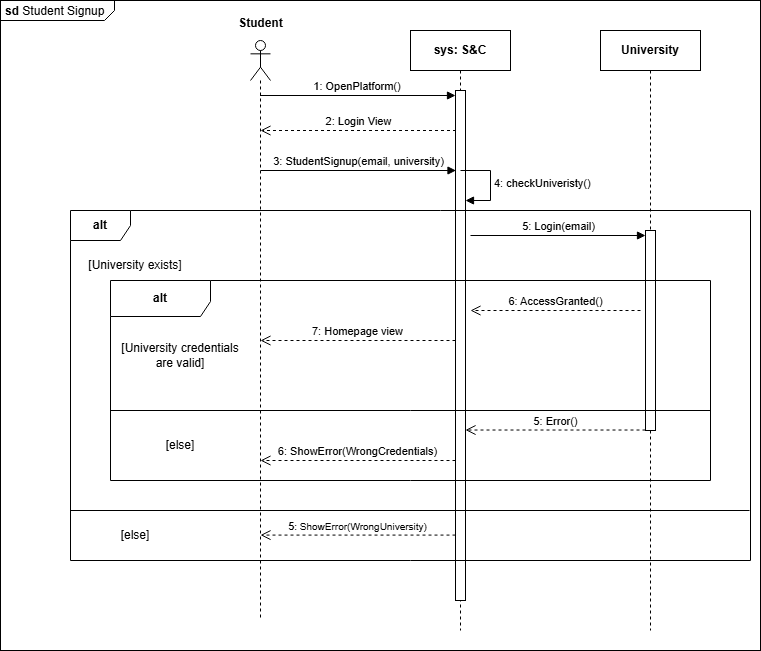
\includegraphics[width=15cm]{Images/UC_diagram/RASD-UC1.png}
    \caption{Students Signup}
\end{figure}

\begin{figure}[H]
\textbf{[UC\nextUCDiagr] Student Log in}\newline\newline
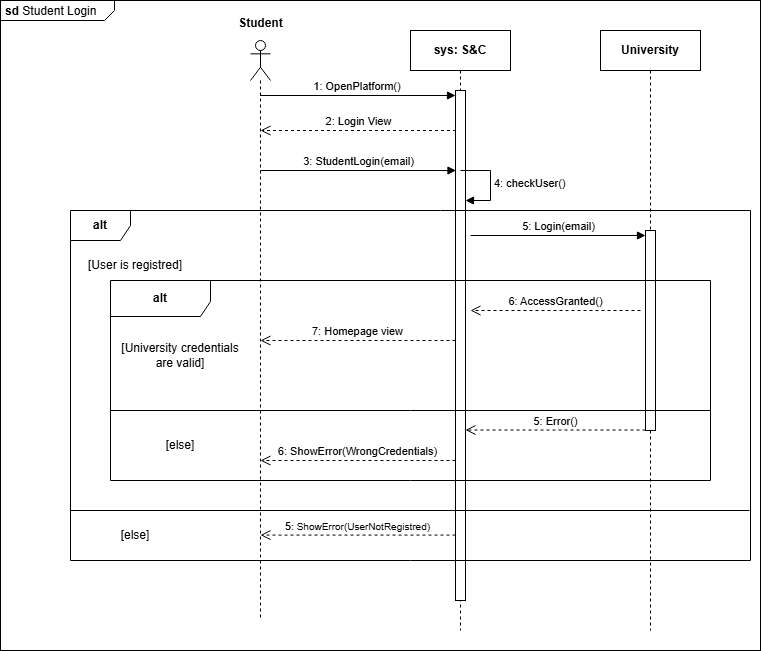
\includegraphics[width=15cm]{Images/UC_diagram/RASD-UC2.drawio.png}
    \caption{Student Log in}
\end{figure}

\begin{figure}[H]
\textbf{[UC\nextUCDiagr] Company Sign up}\newline\newline
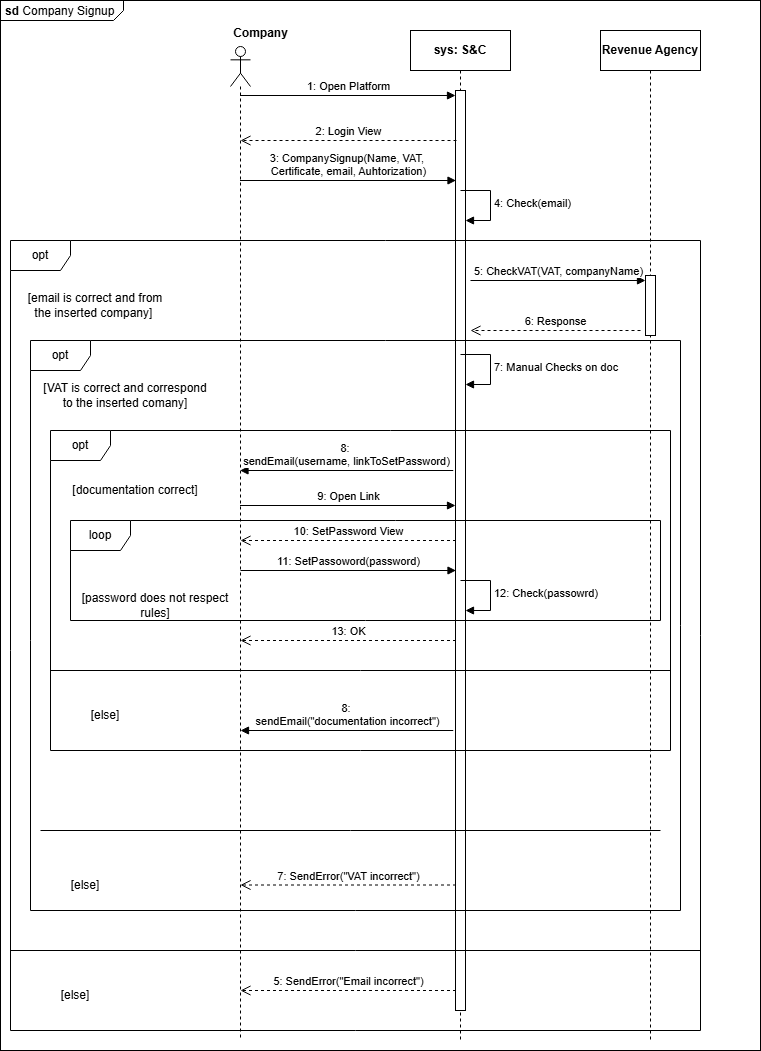
\includegraphics[width=15cm]{Images/UC_diagram/RASD-UC3.drawio.png}
    \caption{Company Sign up}
\end{figure}

\begin{figure}[H]
\textbf{[UC\nextUCDiagr] Company Log in}\newline\newline
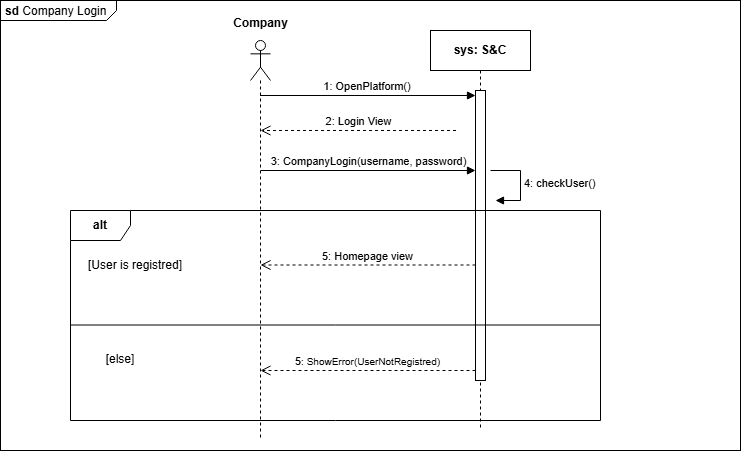
\includegraphics[width=15cm]{Images/UC_diagram/RASD-UC4.drawio.png}
    \caption{Company Log in}
\end{figure}

\begin{figure}[H]
\textbf{[UC\nextUCDiagr] Update Student's CV}\newline\newline
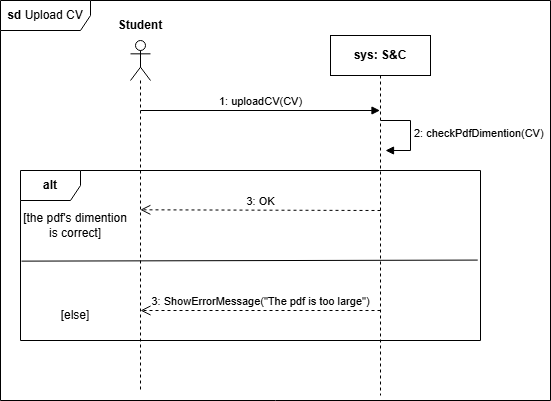
\includegraphics[width=15cm]{Images/UC_diagram/RASD-UC5.drawio.png}
    \caption{Update Student's CV}
\end{figure}

\begin{figure}[H]
\textbf{[UC\nextUCDiagr] Insert Student’s experiences, skills and/or attitudes}\newline\newline
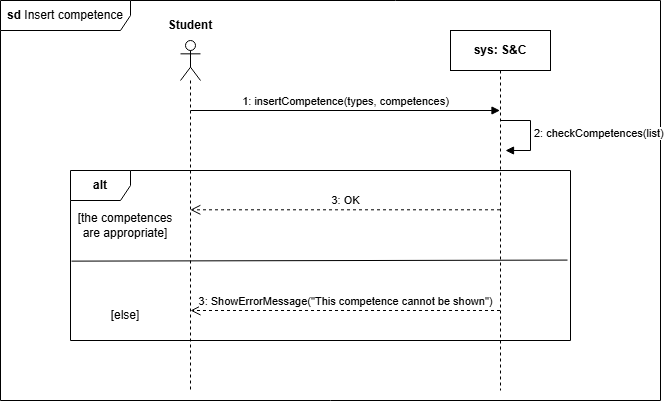
\includegraphics[width=15cm]{Images/UC_diagram/RASD-UC6.drawio.png}
    \caption{Insert Student’s experiences, skills and/or attitudes}
\end{figure}

\begin{figure}[H]
\textbf{[UC\nextUCDiagr] Edit or delete Student’s experiences, skills and/or attitudes}\newline\newline
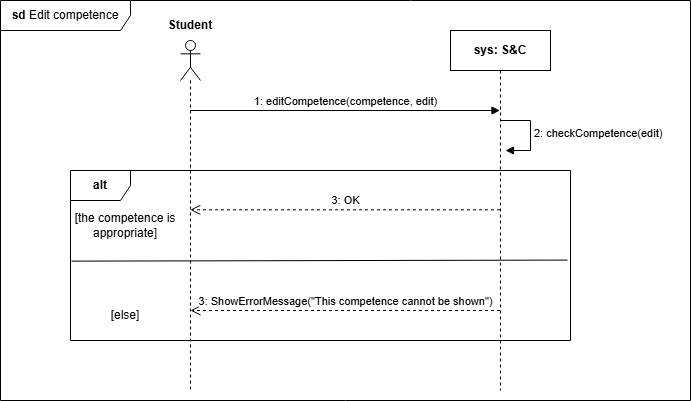
\includegraphics[width=15cm]{Images/UC_diagram/RASD-UC7.drawio.png}
    \caption{Edit or delete Student’s experiences, skills and/or attitudes}
\end{figure}

\begin{figure}[H]
\textbf{[UC\nextUCDiagr] Create internship advertising}\newline\newline
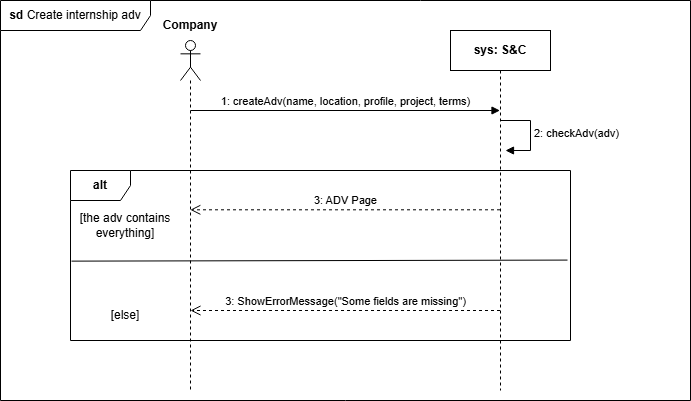
\includegraphics[width=15cm]{Images/UC_diagram/RASD-UC8.drawio.png}
    \caption{Create internship advertising}
\end{figure}

\begin{figure}[H]
\textbf{[UC\nextUCDiagr.1] Edit internship advertising}\newline\newline
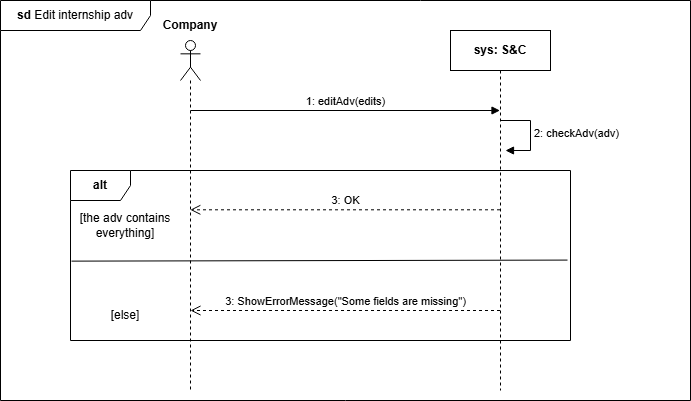
\includegraphics[width=15cm]{Images/UC_diagram/RASD-UC9.drawio.png}
    \caption{Remove internship advertising}
\end{figure}

\begin{figure}[H]
\textbf{[UC9.2] Remove internship advertising}\newline\newline
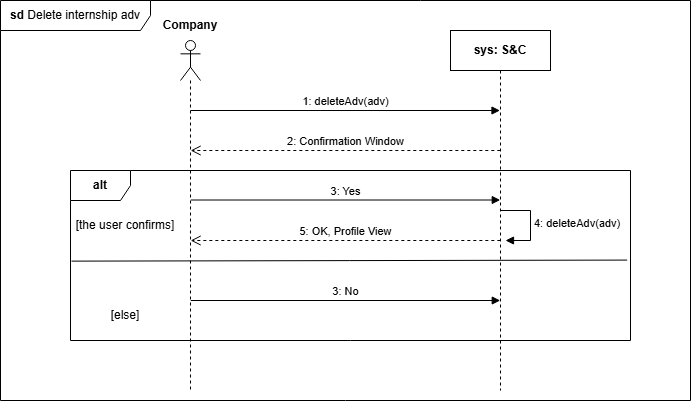
\includegraphics[width=15cm]{Images/UC_diagram/RASD-UC10.drawio.png}
    \caption{Proactive internship research}
\end{figure}

\begin{figure}[H]
\textbf{[UC\nextUCDiagr] Proactive internship research}\newline\newline
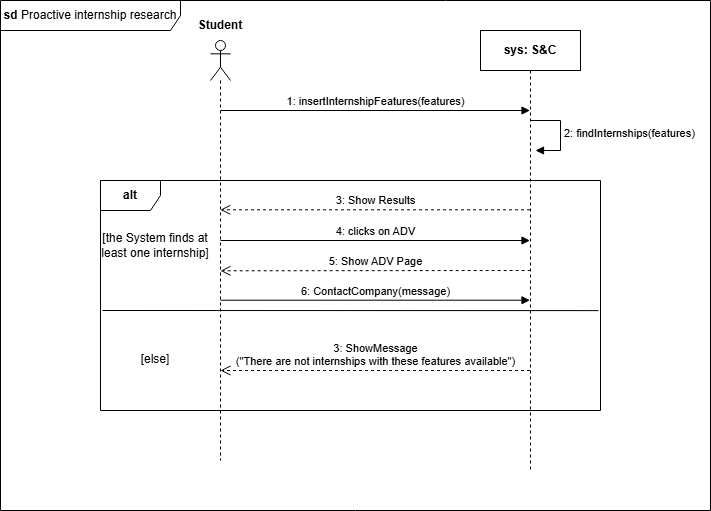
\includegraphics[width=15cm]{Images/UC_diagram/RASD-UC11.drawio.png}
    \caption{Proactive internship research}
\end{figure}

\begin{figure}[H]
\textbf{[UC\nextUCDiagr] Proactive candidates research}\newline\newline
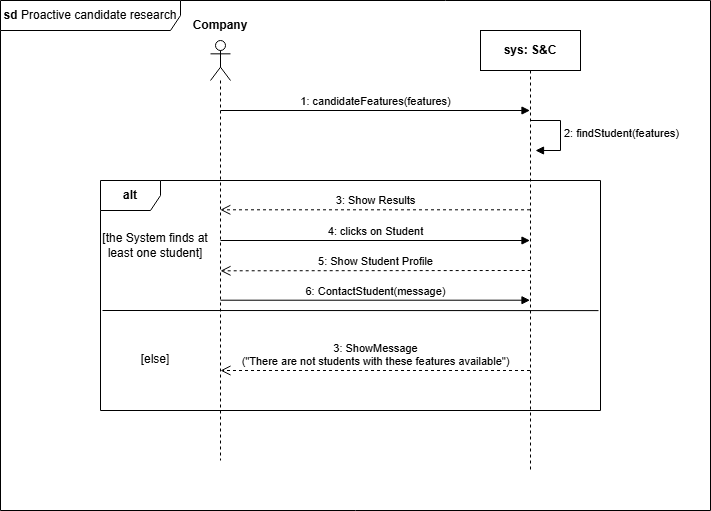
\includegraphics[width=15cm]{Images/UC_diagram/RASD-UC12.drawio.png}
    \caption{Proactive candidates research}
\end{figure}

\begin{figure}[H]
\textbf{[UC\nextUCDiagr-\nextUCDiagr-\nextUCDiagr-\nextUCDiagr] Consult Recommendations}\newline\newline
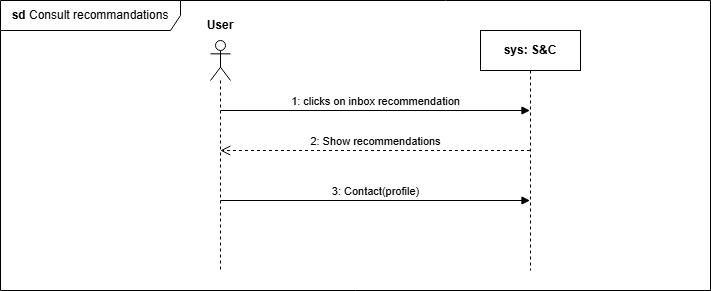
\includegraphics[width=15cm]{Images/UC_diagram/RASD-UC13.drawio.png}
    \caption{Consult Recommendations}
\end{figure}

\begin{figure}[H]
\textbf{[UC\nextUCDiagr.1] Accept internship request (Student)}\newline\newline
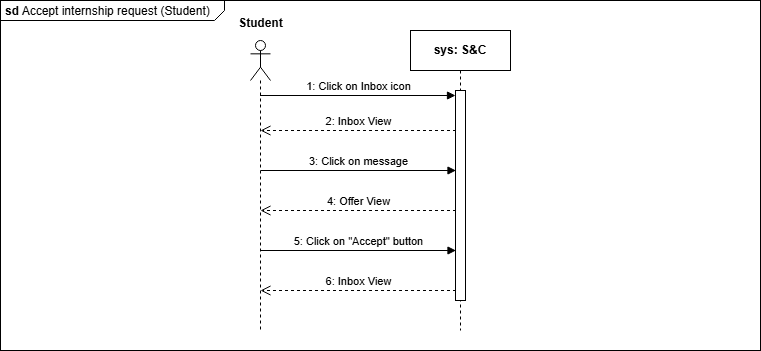
\includegraphics[width=15cm]{Images/UC_diagram/RASD-UC14.drawio.png}
    \caption{Accept internship request (Company)}
\end{figure}

\begin{figure}[H]
\textbf{[UC16.2] Reject internship request (Student)}\newline\newline
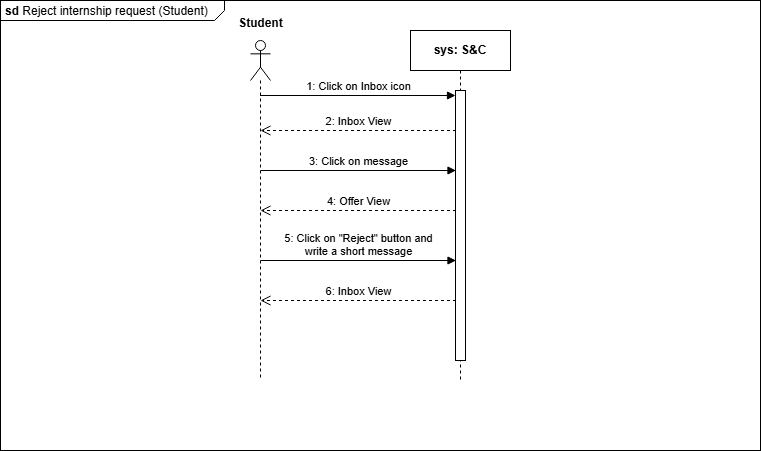
\includegraphics[width=15cm]{Images/UC_diagram/RASD-UC16.drawio.png}
    \caption{Accept internship request (Company)}
\end{figure}

\begin{figure}[H]
\textbf{[UC\nextUCDiagr.1] Accept internship request (Company)}\newline\newline
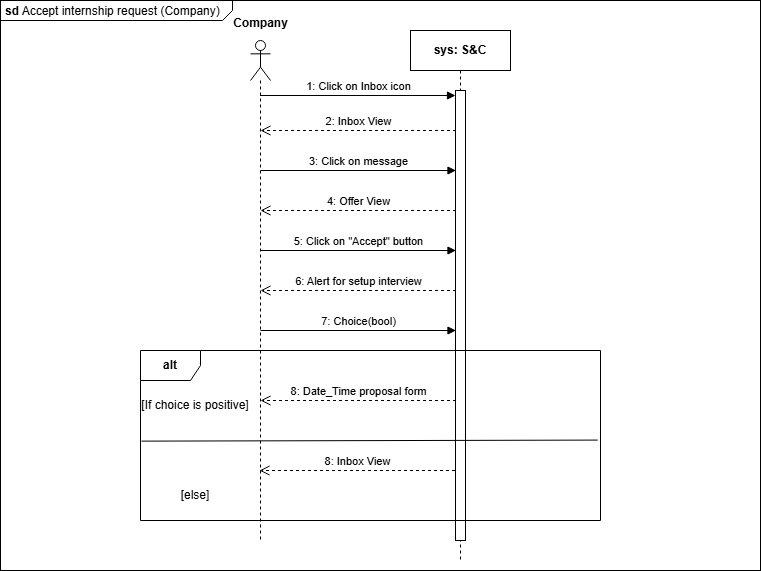
\includegraphics[width=15cm]{Images/UC_diagram/RASD-UC15.drawio.png}
    \caption{Accept internship request (Company)}
\end{figure}

\begin{figure}[H]
\textbf{[UC17.2] Reject internship request (Company)}\newline\newline
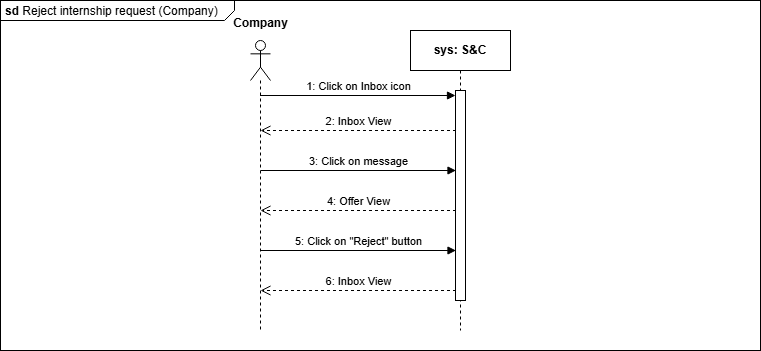
\includegraphics[width=15cm]{Images/UC_diagram/RASD-UC17.drawio.png}
    \caption{Reject internship request (Company)}
\end{figure}

\begin{figure}[H]
\textbf{[UC\nextUCDiagr] Check request outcome (Student)}\newline\newline
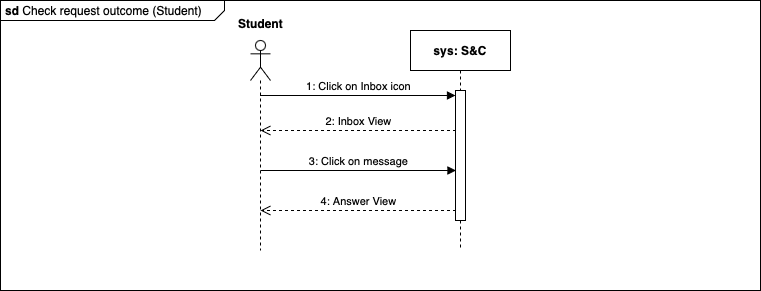
\includegraphics[width=15cm]{Images/UC_diagram/RASD-UC_CheckRequestOutcome(S).png}
    \caption{Check request outcome (Student)}
\end{figure}

\begin{figure}[H]
\textbf{[UC\nextUCDiagr] Check request outcome (Company)}\newline\newline
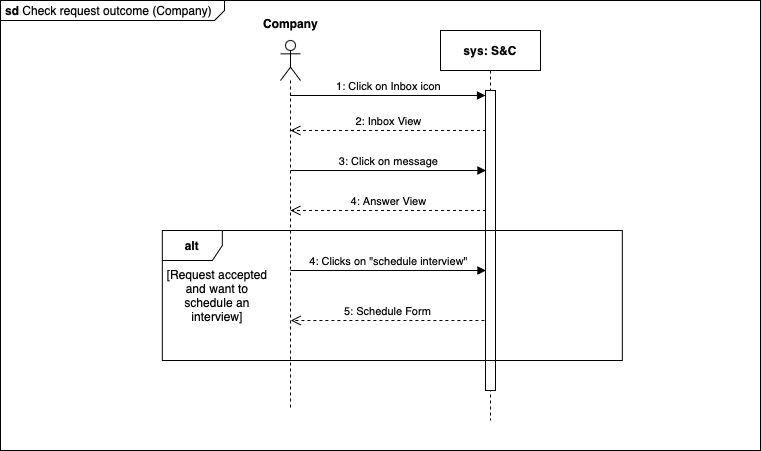
\includegraphics[width=15cm]{Images/UC_diagram/RASD-UC_CheckRequestOutcome(C).png}
    \caption{Check request outcome (Company)}
\end{figure}

\begin{figure}[H]
\textbf{[UC\nextUCDiagr.1] Propose a date for an interview}\newline\newline
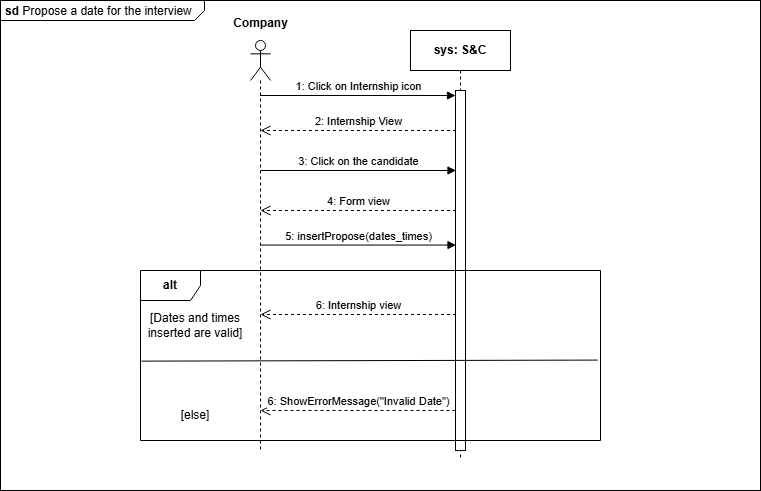
\includegraphics[width=15cm]{Images/UC_diagram/RASD-UC18.drawio.png}
    \caption{Propose a date for an interview}
\end{figure}

\begin{figure}[H]
\textbf{[UC20.2] Accepting a date for an interview}\newline\newline
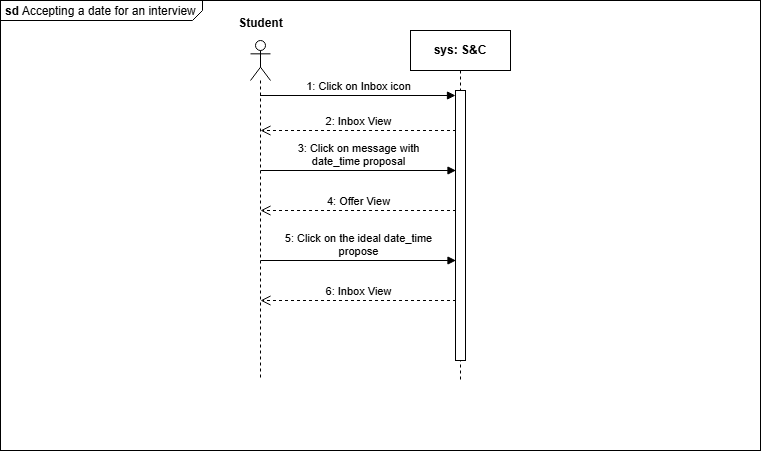
\includegraphics[width=15cm]{Images/UC_diagram/RASD-UC19.drawio.png}
    \caption{Accepting a date for an interview}
\end{figure}

\begin{figure}[H]
\textbf{[UC20.3] Reject a date for an interview}\newline\newline
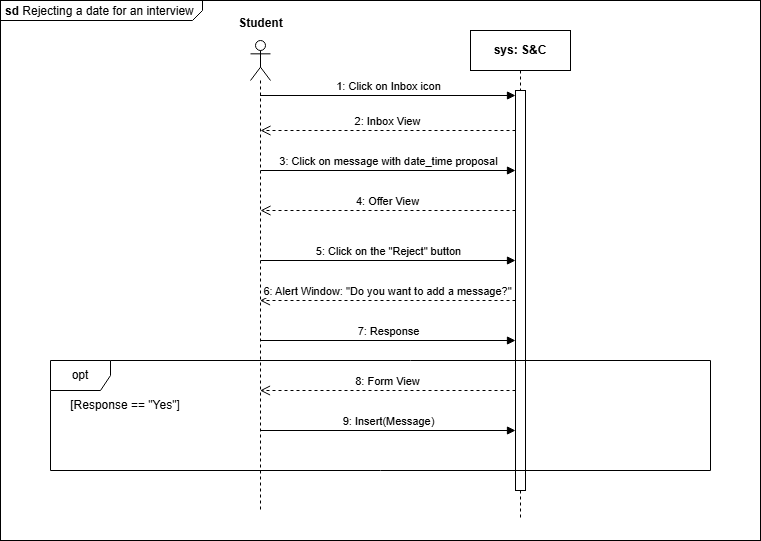
\includegraphics[width=15cm]{Images/UC_diagram/RASD-UC20.drawio.png}
    \caption{Reject a date for an interview}
\end{figure}

\begin{figure}[H]
\textbf{[UC\nextUCDiagr] Creating form for interview}\newline\newline
    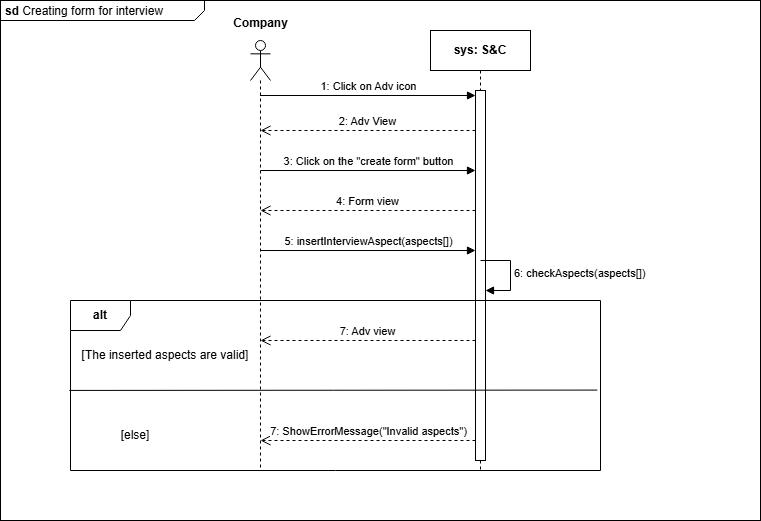
\includegraphics[width=15cm]{Images/UC_diagram/RASD-UC21.drawio.png}
    \caption{Creating form for interview}
\end{figure}

\begin{figure}[H]
\textbf{[UC\nextUCDiagr.1] Deleting form for interview}\newline\newline
    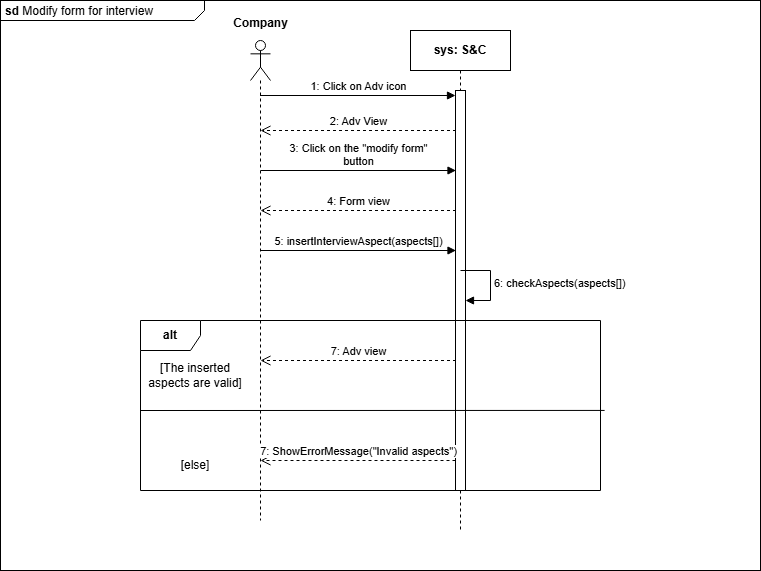
\includegraphics[width=15cm]{Images/UC_diagram/RASD-UC22.drawio.png}
    \caption{Deleting form for interview}
\end{figure}

\begin{figure}[H]
\textbf{[UC22.2 Modify form for interview}\newline\newline
    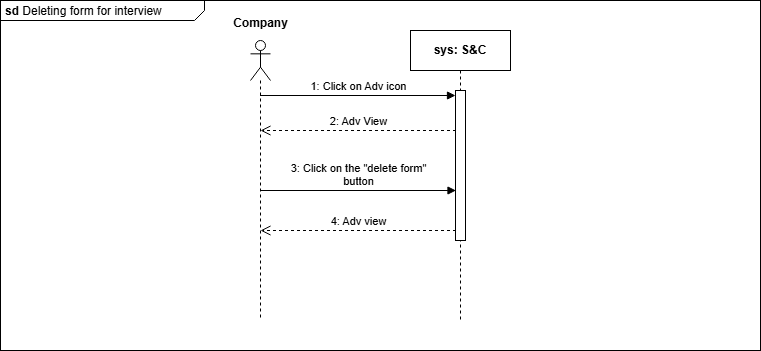
\includegraphics[width=15cm]{Images/UC_diagram/RASD-UC23.drawio.png}
    \caption{Modify form for interview}
\end{figure}

\begin{figure}[H]
\textbf{[UC\nextUCDiagr] Fill the form during interview}\newline\newline
    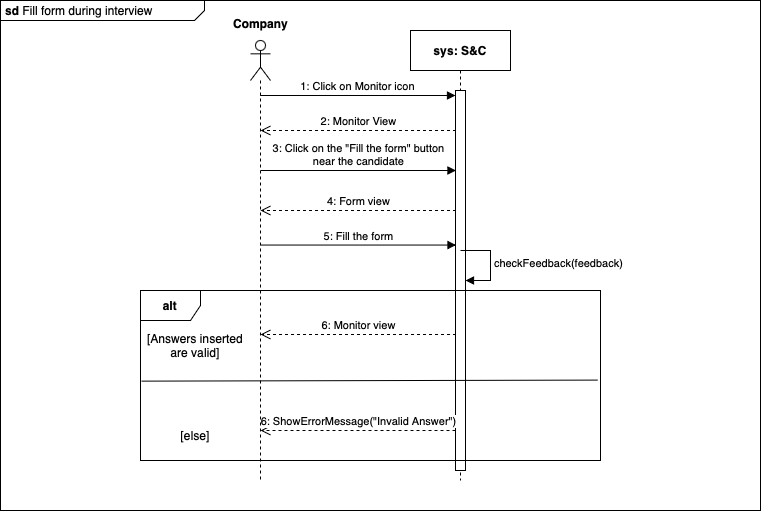
\includegraphics[width=15cm]{Images/UC_diagram/RASD-UC_FillInterviewForm.png}
    \caption{Fill the form during interview}
\end{figure}

\begin{figure}[H]
\textbf{[UC\nextUCDiagr] Feedback (Student)}\newline\newline
    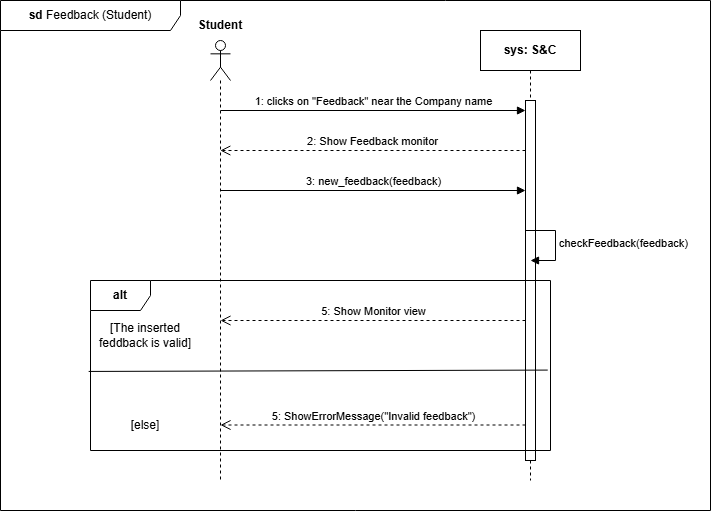
\includegraphics[width=15cm]{Images/UC_diagram/RASD-UC26.drawio.png}
    \caption{Feedback (Student)}
\end{figure}

\begin{figure}[H]
\textbf{[UC\nextUCDiagr] Feedback (Company)}\newline\newline
    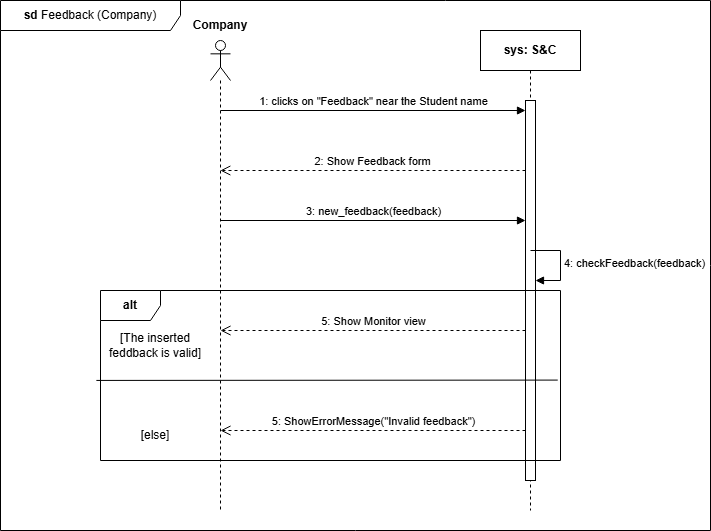
\includegraphics[width=15cm]{Images/UC_diagram/RASD-UC25.drawio.png}
    \caption{Feedback (Company)}
\end{figure}

\begin{figure}[H]
\textbf{[UC\nextUCDiagr-\nextUCDiagr-\nextUCDiagr] Monitoring}\newline\newline
    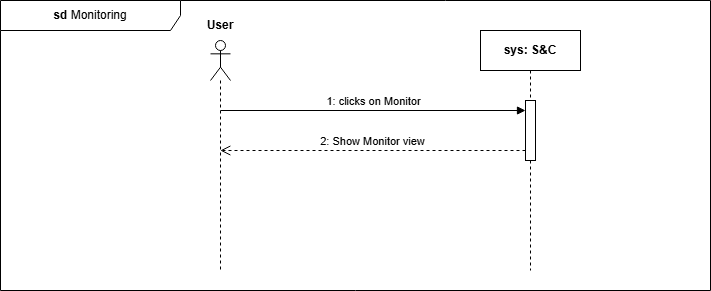
\includegraphics[width=15cm]{Images/UC_diagram/RASD-UC24.drawio.png}
    \caption{Monitoring}
\end{figure}
\subsection{Requirement Mapping}
\subsubsection{Goal-Domain Assumption-Requirement}
\begin{table}[H]
    \centering
    \begin{tabular}{|p{15cm}|}
    \hline
    {\textbf{[G1]} University students can find companies aligned with their interests, apply for internships, complete interviews, and track every stage of the process, from application to the successful completion of the internship.} \\ \hline
    \begin{itemize}
        \item[\text{[D1]}] Companies offers real internship positions.
        \item[\text{[D2]}] Students search for internship related to their course.
        \item[\text{[D3]}] Students write their CV according to their real experiences, skills and attitudes.
        \item[\text{[D4]}] The experiences, skills, and attitudes shown in the students' profiles are consistent with those in their respective CVs.
        \item[\text{[D5]}] Companies are honest in listing the projects and the terms offered.
        \item[\text{[D6]}] Students and companies are honest when giving feedback.
        \item[\text{[D7]}] Students and companies have access to a working Internet connection.
        \item[\text{[D8]}] Employees of the S\&C platform that checks the validity of a Company are capable and honest.
    \end{itemize}
    \\\hline 
    \begin{itemize}
        \item[\text{[R1]}] S\&C allows Students to sign up to the platform through their university credentials using SSO access.
        \item[\text{[R2]}] S\&C allows Student to login via their university credentials.
        \item[\text{[R5]}] S\&C allows Students to upload the PDF of their CV (both for the first time and other times if there have been some changes).
        \item[\text{[R6]}] S\&C allows Students to insert new experiences, skills, and attitudes on their profile.
        \item[\text{[R7]}] S\&C allows Students to edit or delete experiences, skills, and attitudes present on their profile.
        \item[\text{[R10]}] S\&C allows Students to use a research bar to find appropriate internship positions by inserting specific requirements about the project and/or the terms offered.
        \item [\text{[R12]}] S\&C informs students when an internship that might interest them becomes available.
        \item [\text{[R14]}] S\&C allows Students to contact a Company they are interested in.
        \item [\text{[R16]}] S\&C informs a Student when a Company shows interest in their profile by sending the Student the Company's offer. The Student can accept or decline the offer.
        \item [\text{[R18]}] S\&C communicates to Students or Companies if their requests are successful.
        \item [\text{[R19]}] S\&C allows Companies to setup an interview with the candidates.
        \item [\text{[R24]}] S\&C allows Companies to give feedback during the internship about a single Student.
        \item [\text{[R25]}] S\&C offers Students the possibility to monitor their matchmaking process with a Company (state of the matchmaking, scheduled interview, interview results).
        \item [\text{[R27]}] S\&C offers Students and Companies the possibility to monitor the state of the internship.
    \end{itemize}
    
    \\ \hline
    \end{tabular}
\end{table}

\begin{table}[H]
    \centering
    \begin{tabular}{|p{15cm}|}
    \hline
    {\textbf{[G2]} Companies can advertise their internship opportunities to find suitable students for the position, contact them, conduct interviews, hire the best candidates, and keep track of the entire process.} 
    \\\hline \begin{itemize}
        \item[\text{[D3]}] Students write their CVs according to their real experiences, skills and attitudes.
        \item[\text{[D4]}] The experiences, skills, and attitudes shown in the students' profiles are consistent with those in their respective CVs. 
        \item[\text{[D6]}] Students and companies are honest when giving feedback.
        \item[\text{[D7]}] Students and companies have access to a working Internet connection.
    \end{itemize}\\ \hline
    \begin{itemize}
         \item[\text{[R3]}] S\&C allows Companies to sign up to the platform by asking the representative of the company to insert their company email, the VAT number of the company, a Certificate of registration at the Chamber of Commerce, and a letter of authorisation or official assignment signed by a CEO or a HR referent. They have to choose a password.
        \item[\text{[R4]}] S\&C allows Companies to login to the platform via password and username (created by the system).
        \item[\text{[R8]}] S\&C allows Companies to create an advertisement regarding an internship position they are offering, explaining the project of the internship and the terms offered.
    
        \item[\text{[R9]}] S\&C allows Companies to modify and remove an advertisement posted on their page.
        \item[\text{[R11]}] S\&C allows Companies to use a research bar to find appropriate candidates for their internship positions by inserting specific experiences, skills and/or attitudes the candidates should have.
        \item [\text{[R13]}] S\&C informs companies about the availability of a student whose CV corresponds to their needs.
        \item [\text{[R14]}] S\&C allows Students to contact a Company they are interested in.
        \item [\text{[R15]}] S\&C allows Companies to contact Students they are interested in.
        \item [\text{[R16]}] S\&C informs a Student when a Company shows interest in their profile by sending the Student the Company's offer. The Student can accept or decline the offer.
    
        \item [\text{[R17]}] S\&C informs a Company when a Student shows interest in its offer by sending to the Company the Student's CV, the Company can accept or decline the offer.
    
        \item [\text{[R18]}] S\&C communicates to Students or Companies if their requests are successful.
    \item [\text{[R19]}] S\&C allows Companies to setup an interview with the candidates.
    
        \item [\text{[R20]}] S\&C allows Companies to write a form with all the aspects that will be considered during the interviews.
    
        \item [\text{[R21]}] S\&C allows Companies to modify or delete the interview form created.
        \item [\text{[R22]}] S\&C allows Companies fill the form during the interview.
        \item [\text{[R23]}] S\&C allows Students to give personal feedback during the selection period about the Company's selection method or during the internship period about the internship itself.
        \item [\text{[R26]}] S\&C offers Companies the possibility to monitor their matchmaking process with a Student.
    
        \item [\text{[R27]}] S\&C offers Students and Companies the possibility to monitor the state of the internship.
    \end{itemize}
     \\ \hline
    \end{tabular}
\end{table}

\subsubsection{Requirement - Use Case}
\begin{table}[H]
    \centering
    \begin{tabular}{|p{10cm}|p{5cm}|}
    \hline
         [R1] S\&C allows Students to sign up to the platform through their university credentials using SSO access. & [UC1] Students Signup \\ \hline
         [R2] S\&C allows Student to login via their university credentials.& [UC2] Students Login\\\hline
         [R3] S\&C allows Companies to sign up to the platform by asking the representative of the company to insert their company email, the VAT number of the company, a Certificate of registration at the Chamber of Commerce, and a letter of authorisation or official assignment signed by a CEO or a HR referent. They have to choose a password. &[UC3] Company Sign up \\\hline
         [R4] S\&C allows Companies to login to the platform via password and username (created by the system). & [UC4] Company Login\\\hline
         [R5] S\&C allows Students to upload the PDF of their CV (both for the first time and other times if there have been some changes).[UC5] Update student’s CV & [UC5] Update student’s CV\\\hline
         [R6] S\&C allows Students to insert new experiences, skills, and attitudes on their profile.& [UC6] Insert Student’s experiences, skills and/or attitudes\\\hline
         [R7] S\&C allows Students to edit or delete experiences, skills, and attitudes present on their profile.&[UC7] Edit or delete Student’s experiences, skills and/or attitudes \\\hline
         [R8] S\&C allows Companies to create an advertisement regarding an internship position they are offering, explaining the project of the internship and the terms offered. &[UC8] Create internship advertising \\\hline
         [R9] S\&C allows Companies to modify and remove an advertisement posted on their page.&[UC9.1] Edit internship advertising\newline[UC9.2] Remove internship advertising \\\hline
         [R10] S\&C allows Students to use a research bar to find appropriate internship positions by inserting specific requirements about the project and/or the terms offered. & [UC10] Proactive internship research \\\hline
         [R11] S\&C allows Companies to use a research bar to find appropriate candidates for their internship positions by inserting specific experiences, skills and/or attitudes the candidates should have. & [UC11] Proactive candidates research\\\hline
         [R12] S\&C informs students when an internship that might interest them becomes available. \newline [R13] S\&C informs companies about the availability of a student whose CV corresponds to their needs. \newline [R14] S\&C allows Students to contact a Company they are interested in. \newline [R15] S\&C allows Companies to contact Students they are interested in. & [UC12-13-14-15] Consult Recommendations\\\hline
     \end{tabular}
\end{table}
\begin{table}[H]
    \centering
    \begin{tabular}{|p{10cm}|p{5cm}|}
    \hline
         [R16]  S\&C informs a Student when a Company shows interest in their profile by sending the Student the Company's offer. The Student can accept or decline the offer. & [UC16.1] Accept internship request (Student) \newline [UC16.2] Reject internship request (Student)\\\hline
         [R17] S\&C informs a Company when a Student shows interest in its offer by sending to the Company the Student's CV, the Company can accept or decline the offer. & [UC17.1] Accept internship request (Company) \newline [UC17.2] Reject internship request (Company) \\\hline
         [R18] S\&C communicates to Students or Companies if their requests are successful. &[UC18.1] Check request outcome (Student)\newline [UC18.2] Check request outcome (Company)\\\hline
         [R19] S\&C allows Companies to setup an interview with the candidates. & [UC19.1] Propose a date for an interview\newline [UC19.2] Accepting a date for an interview\newline[UC19.3] Reject a date for an interview \\\hline
         [R20] S\&C allows Companies to write a form with all the aspects that will be considered during the interviews.& [UC20] Creating form for interview\\\hline
         [R21] S\&C allows Companies to modify or delete the interview form created. & [UC21.1] Deleting form for interview \newline [UC21.2] Modify form for interview\\\hline
         [R22] S\&C allows Companies fill the form during the interview. & [UC22] Fill the form for interview\\\hline
         [R23] S\&C allows Students to give personal feedback during the selection period about the Company's selection method or during the internship period about the internship itself. & [UC23] Feedback (Student)\\\hline
         [R24] S\&C allows Companies to give feedback during the internship about a single Student. & [UC24] Feedback (Company)\\\hline
         [R25] S\&C offers Students the possibility to monitor their matchmaking process with a Company (state of the matchmaking, scheduled interview, interview results).\newline [R26] S\&C offers Companies the possibility to monitor their matchmaking process with a Student.\newline S\&C offers Students and Companies the possibility to monitor the state of the internship. & [UC25-26-27] Monitoring\\\hline
    \end{tabular}
\end{table}
\section{Performance Requirements}
\subsection{Number of Users}
In Italy, in 2022, approximately 173 000 university students participated in internships. There are 40,000 Italian companies registered on LinkedIn, and about 70\% of them (equivalent to 28 000) offer internship opportunities to university students. Therefore, the total number of potential users for a website like S\&C in Italy could be around 201 000. Our platform could capture 30\% of this audience, which amounts to approximately \textbf{60 000 users}.
\subsection{Data Storage}
Here is the amount of storage needed categorised:
\begin{itemize}
    \item \textbf{Student's profile}: we consider the average case in which the student uploads the PDF of their CV (maximum 1 MB) and about 10 competences. For each competence, we have to store name (string of length 15/20 chars, i.e. 16-21 bytes), type (char: S-skill, E-experience, A- attitude, i.e. 1 byte), and small description (text of about 2 lines, i.e. 161 bytes), plus an overhead of 7-14 bytes, so, one competence takes up about 191 bytes, consequentially, 10 competences take up about 1,9 KB. We have also to consider the email and the name of the university, both around 35 bytes. So, in total, the storage of the personal information of a student takes up about 1001,97 KB, i.e. 1 MB.
    \item \textbf{Company's profile and ADVs}: for each company, we store the name (string of length 40/50 chars, i.e. 41-51 bytes), the VAT number (11 chars, i.e. 11 bytes), representative's email (35 bytes), password (SHA-256, i.e. 64 chars, i.e. 64 bytes), Certificate of registration at the Chamber of Commerce (500 KB). On average each company could have about 3 Internship Advertisements. For each ADV, we have to store: name (string of length 40/50 chars, i.e. 41-51 bytes), location (30 bytes), candidate profile (500 bytes), project description (1000 bytes), terms offered (500 bytes), interview form (it depends on the amount of fields, on average 3.4 KB). So, for an average company we need about 517 KB.
    \item \textbf{Matches and Recommendations}: both are linked to the users and ADVs involved (so we need their IDs, i.e. 4 bytes each); the matches contain also the status (recognised by a char, so 1 byte). So for a match, we need about 9 bytes, and for a recommendation about 8 bytes. 
    \item \textbf{Feedback}: it will have the IDs of the users involved (8 bytes in total), the comment (about 500 bytes), and the fields regarding the checks to be done on the user profile (about 300 bytes). In total, about 800 bytes.
\end{itemize}
\subsection{Time Response}
Each operation performed by the S\&C platform should be completed within milliseconds, except for the manual control of company registrations.
\section{Design Constraints}
\subsection{Standards Compliance}
The S\&C platform ensures compliance with GDPR (General Data Protection Regulation) for data protection, WCAG (Web Content Accessibility Guidelines) for accessibility, and OWASP (Open Web Application Security Project) to prevent security issues. It uses W3C standards (World Wide Web Consortium) for compatibility and responsive design to support all devices. It implements HTTPS for safe communication and follows ISO/IEC 27001 (Information Security Management) to protect data effectively.
\subsection{Hardware Limitation}
The only limitation for the device concerns the internet connection and a portable device which supports the app or a computer with a Web Browser.
\section{Software System Attributes}
\subsection{Reliability}
The system implements reliability with robust error handling and automatic retries for unsuccessful API calls. 
\subsection{Availability}
The platform is always accessible, maintaining a high availability targeting a 99.9\% uptime ("three nines"), this way the system will be unavailable only for 8.76 hours per year. It uses load balancing to handle high traffic efficiently.
\subsection{Security}
The system must control the User access (Company and Student), verify identity through university credentials for Students and insert VAT number and upload a certificate of the Chamber of Commerce for Companies. Some measure to protect the databases, with all the information, will be adopted, like encryption of personal data and protection against query injections.
\subsection{Maintainability}
The system requires manual intervention only for authorizing Companies Sign up. The ordinary maintenance has to be scheduled during nighttime in order to guarantee the maximum uptime.
\subsection{Portability}
The system is a web application so it must be viewable on different web browsers and devices with different screen proportions.